\begin{figure}[htbp]
  \centering
  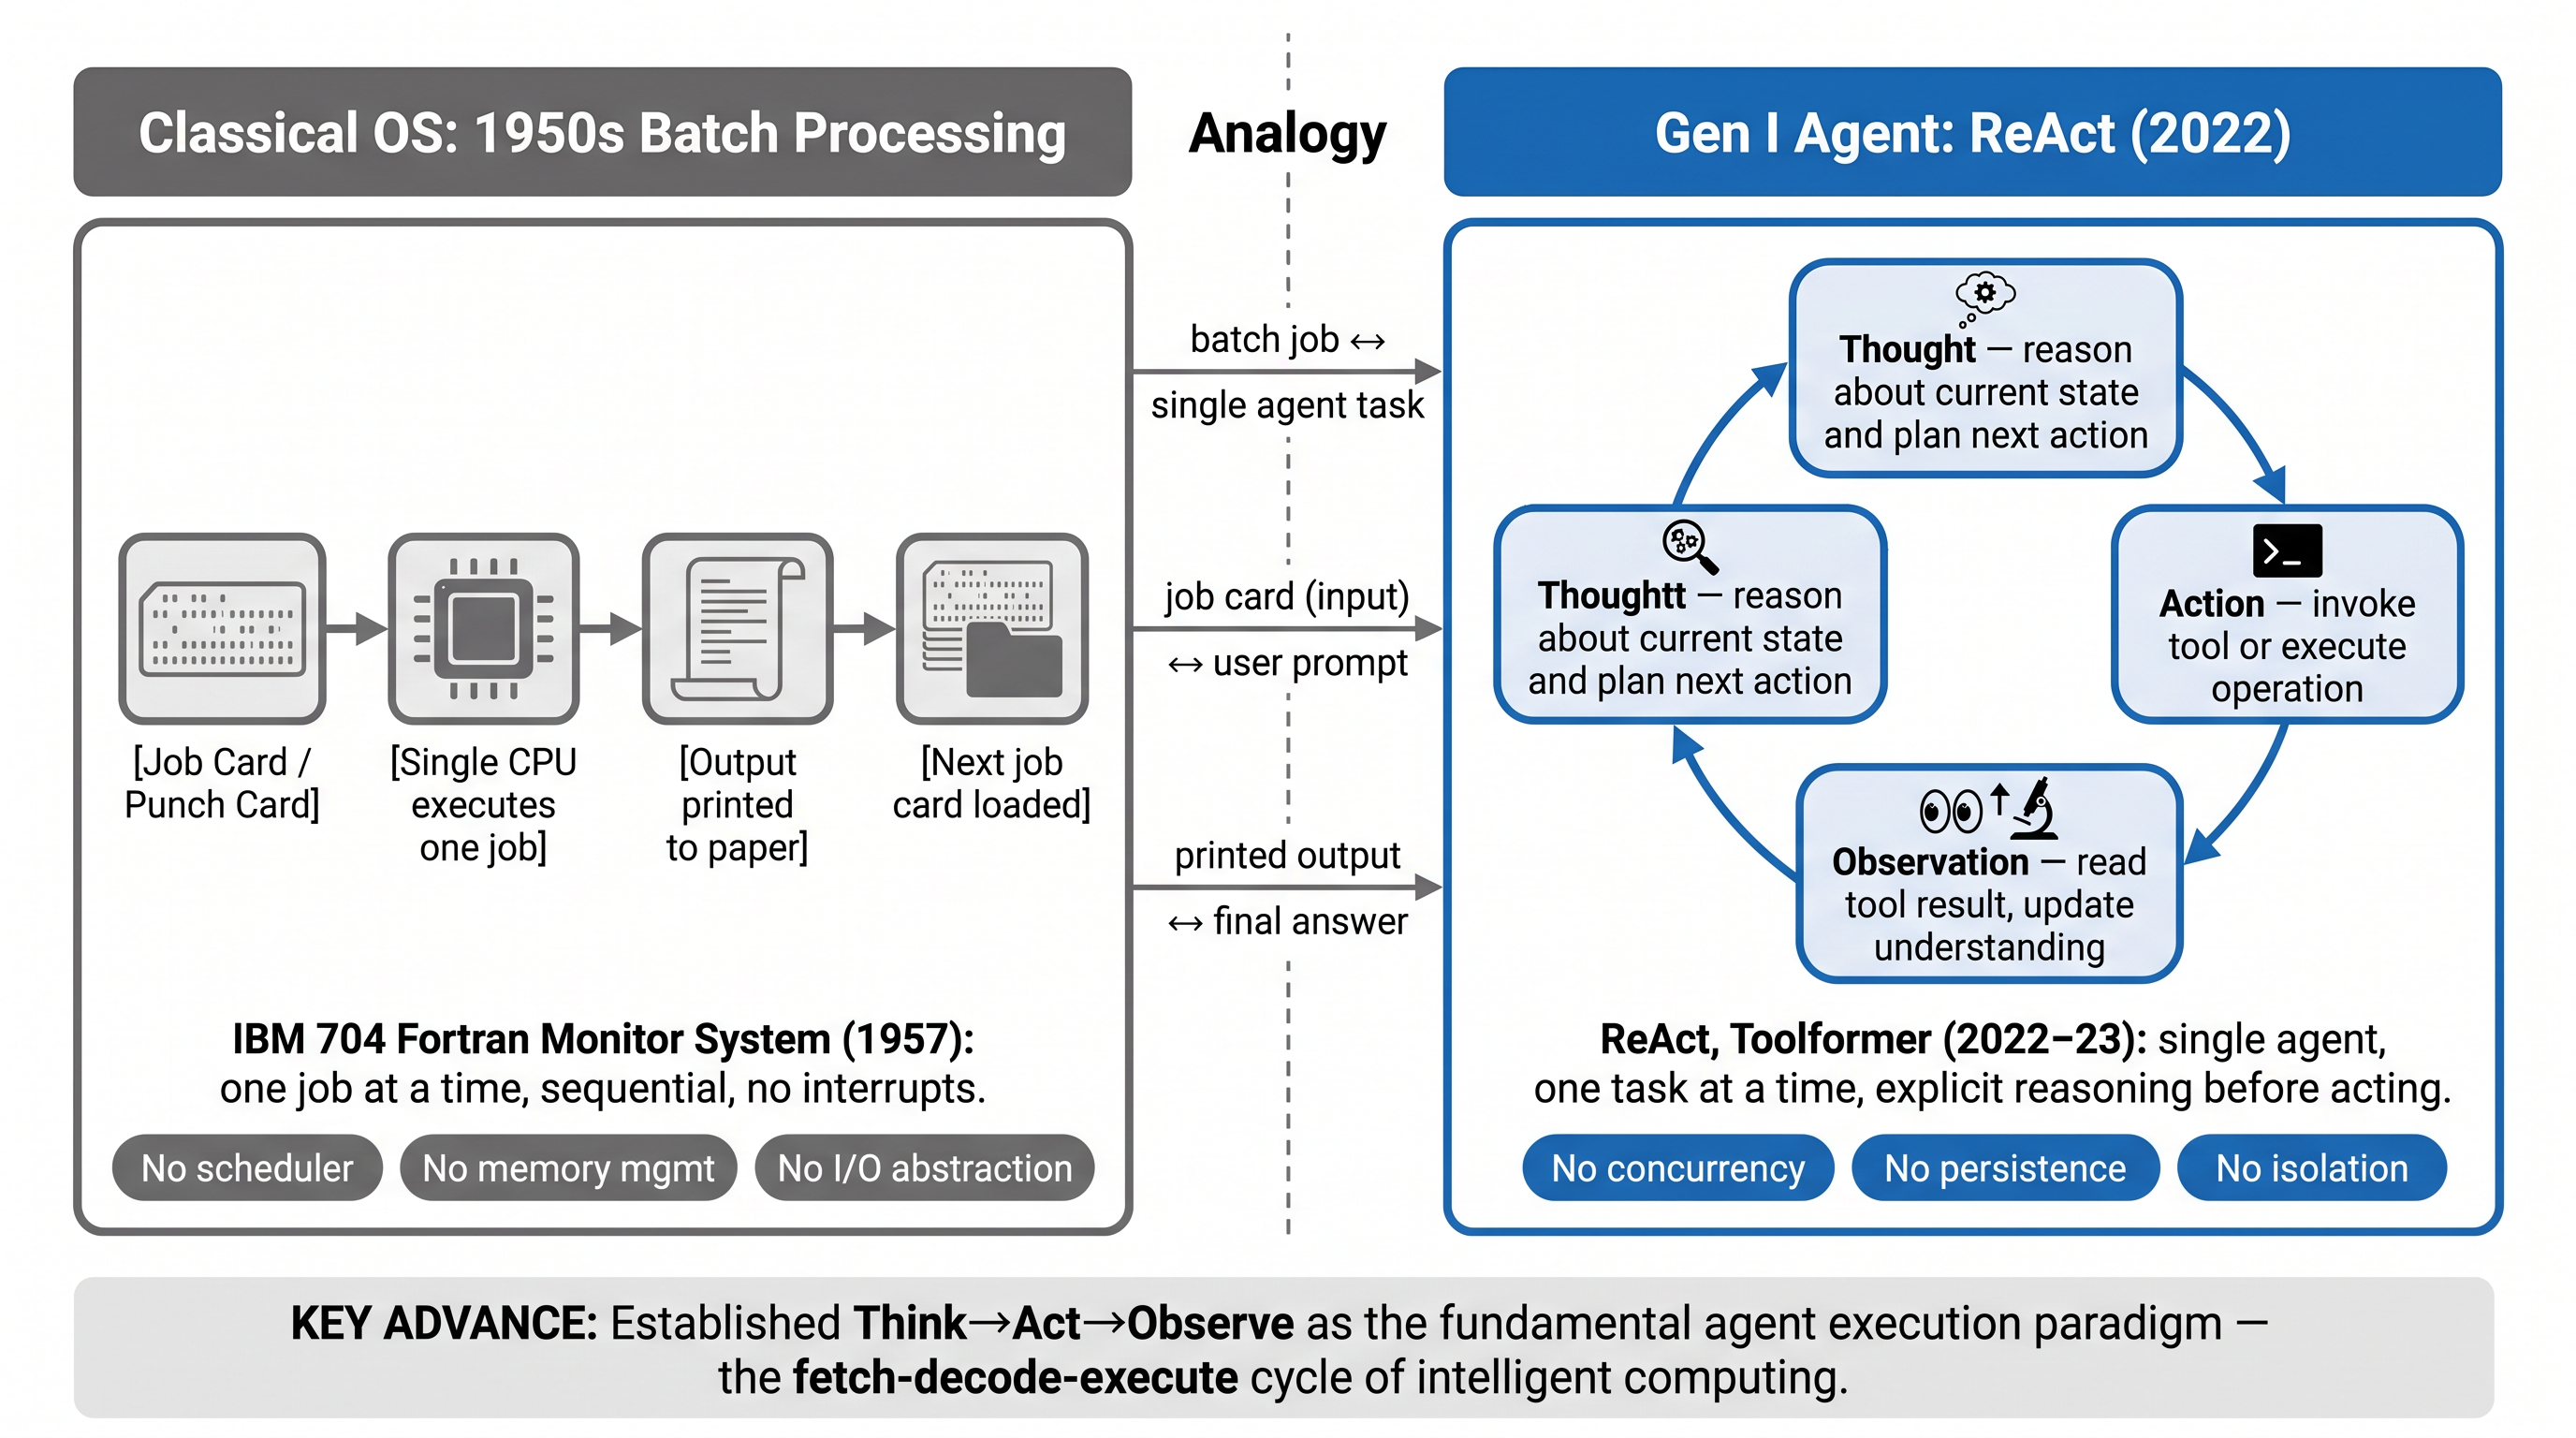
\includegraphics[width=0.88\textwidth]{figures/generated/fig_ae_gen1}
  \caption{Generation~I agent frameworks versus 1950s batch-processing systems.
  The ReAct Think--Act--Observe loop is structurally analogous to a single-job batch system:
  one task executes to completion with no concurrency, no persistent state, and no resource isolation.
  The core advance was establishing the interleaved reasoning--action paradigm
  as the fundamental agent execution primitive.}
  \label{fig:ae:gen1}
\end{figure}
